\documentclass{article}
\usepackage{graphicx}
\usepackage{float}
\usepackage{subcaption}

\begin{document}
\title{Study of two Raspberry Pis and Power adapters}
\author{Abhinav Narain}
\maketitle
\section{Raspberry Pi and Power Adapters}
\subsection{Compare EMI of two power adapters}
\begin{figure}[H]
\centering
\begin{subfigure}{\textwidth}
    \centering
    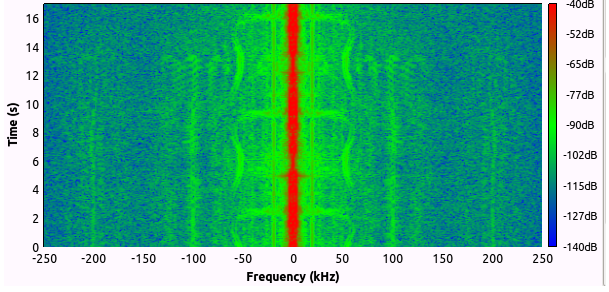
\includegraphics[width=\textwidth]{./figures/raspi-with-usb.png}
    \vspace{-25pt}
    \caption{EMI generated by Raspberry Pi-2 with USB power chord (1)}
    \label{fig:u0}
    \end{subfigure}

    \begin{subfigure}{\textwidth}
    \centering
    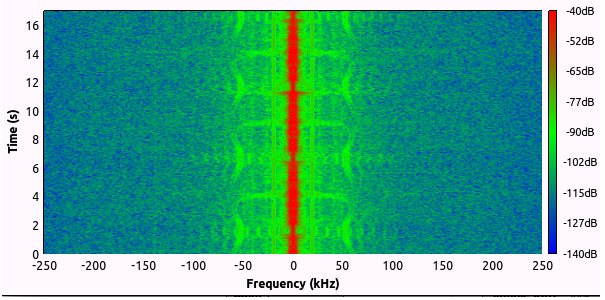
\includegraphics[width=\textwidth]{./figures/raspi-without-usb.png}
    \caption{EMI generated by Raspberry Pi-2 with different power-chord (2)}
        \label{fig:u1}
        \end{subfigure}
   \caption{Same Raspberry Pi-2 shows two different EMI signatures for two different power-chords}
    \label{fig:u2}
\end{figure}

\subsection{Compare EMI of two Raspberry Pis}
\begin{figure}[H]
\centering
\begin{subfigure}{\textwidth}
    \centering
    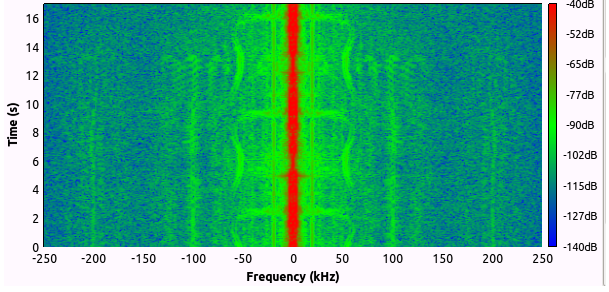
\includegraphics[width=\textwidth]{./figures/raspi-with-usb.png}
    \vspace{-25pt}
    \caption{EMI generated by Raspberry 2 with USB power chord (1)}
    \label{fig:g0}
    \end{subfigure}

    \begin{subfigure}{\textwidth}
    \centering
    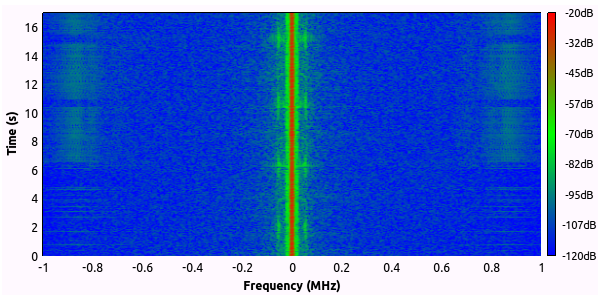
\includegraphics[width=\textwidth]{./figures/raspi-old.png}
    \caption{EMI generated by Raspberry 1 with USB power chord (1)}
        \label{fig:g1}
        \end{subfigure}
   \caption{Two different Raspberry Pi using the same power chord but have different EMI signatures }
    \label{fig:g2}
\end{figure}

\section{Miscellaneous}

\begin{figure}[H]
    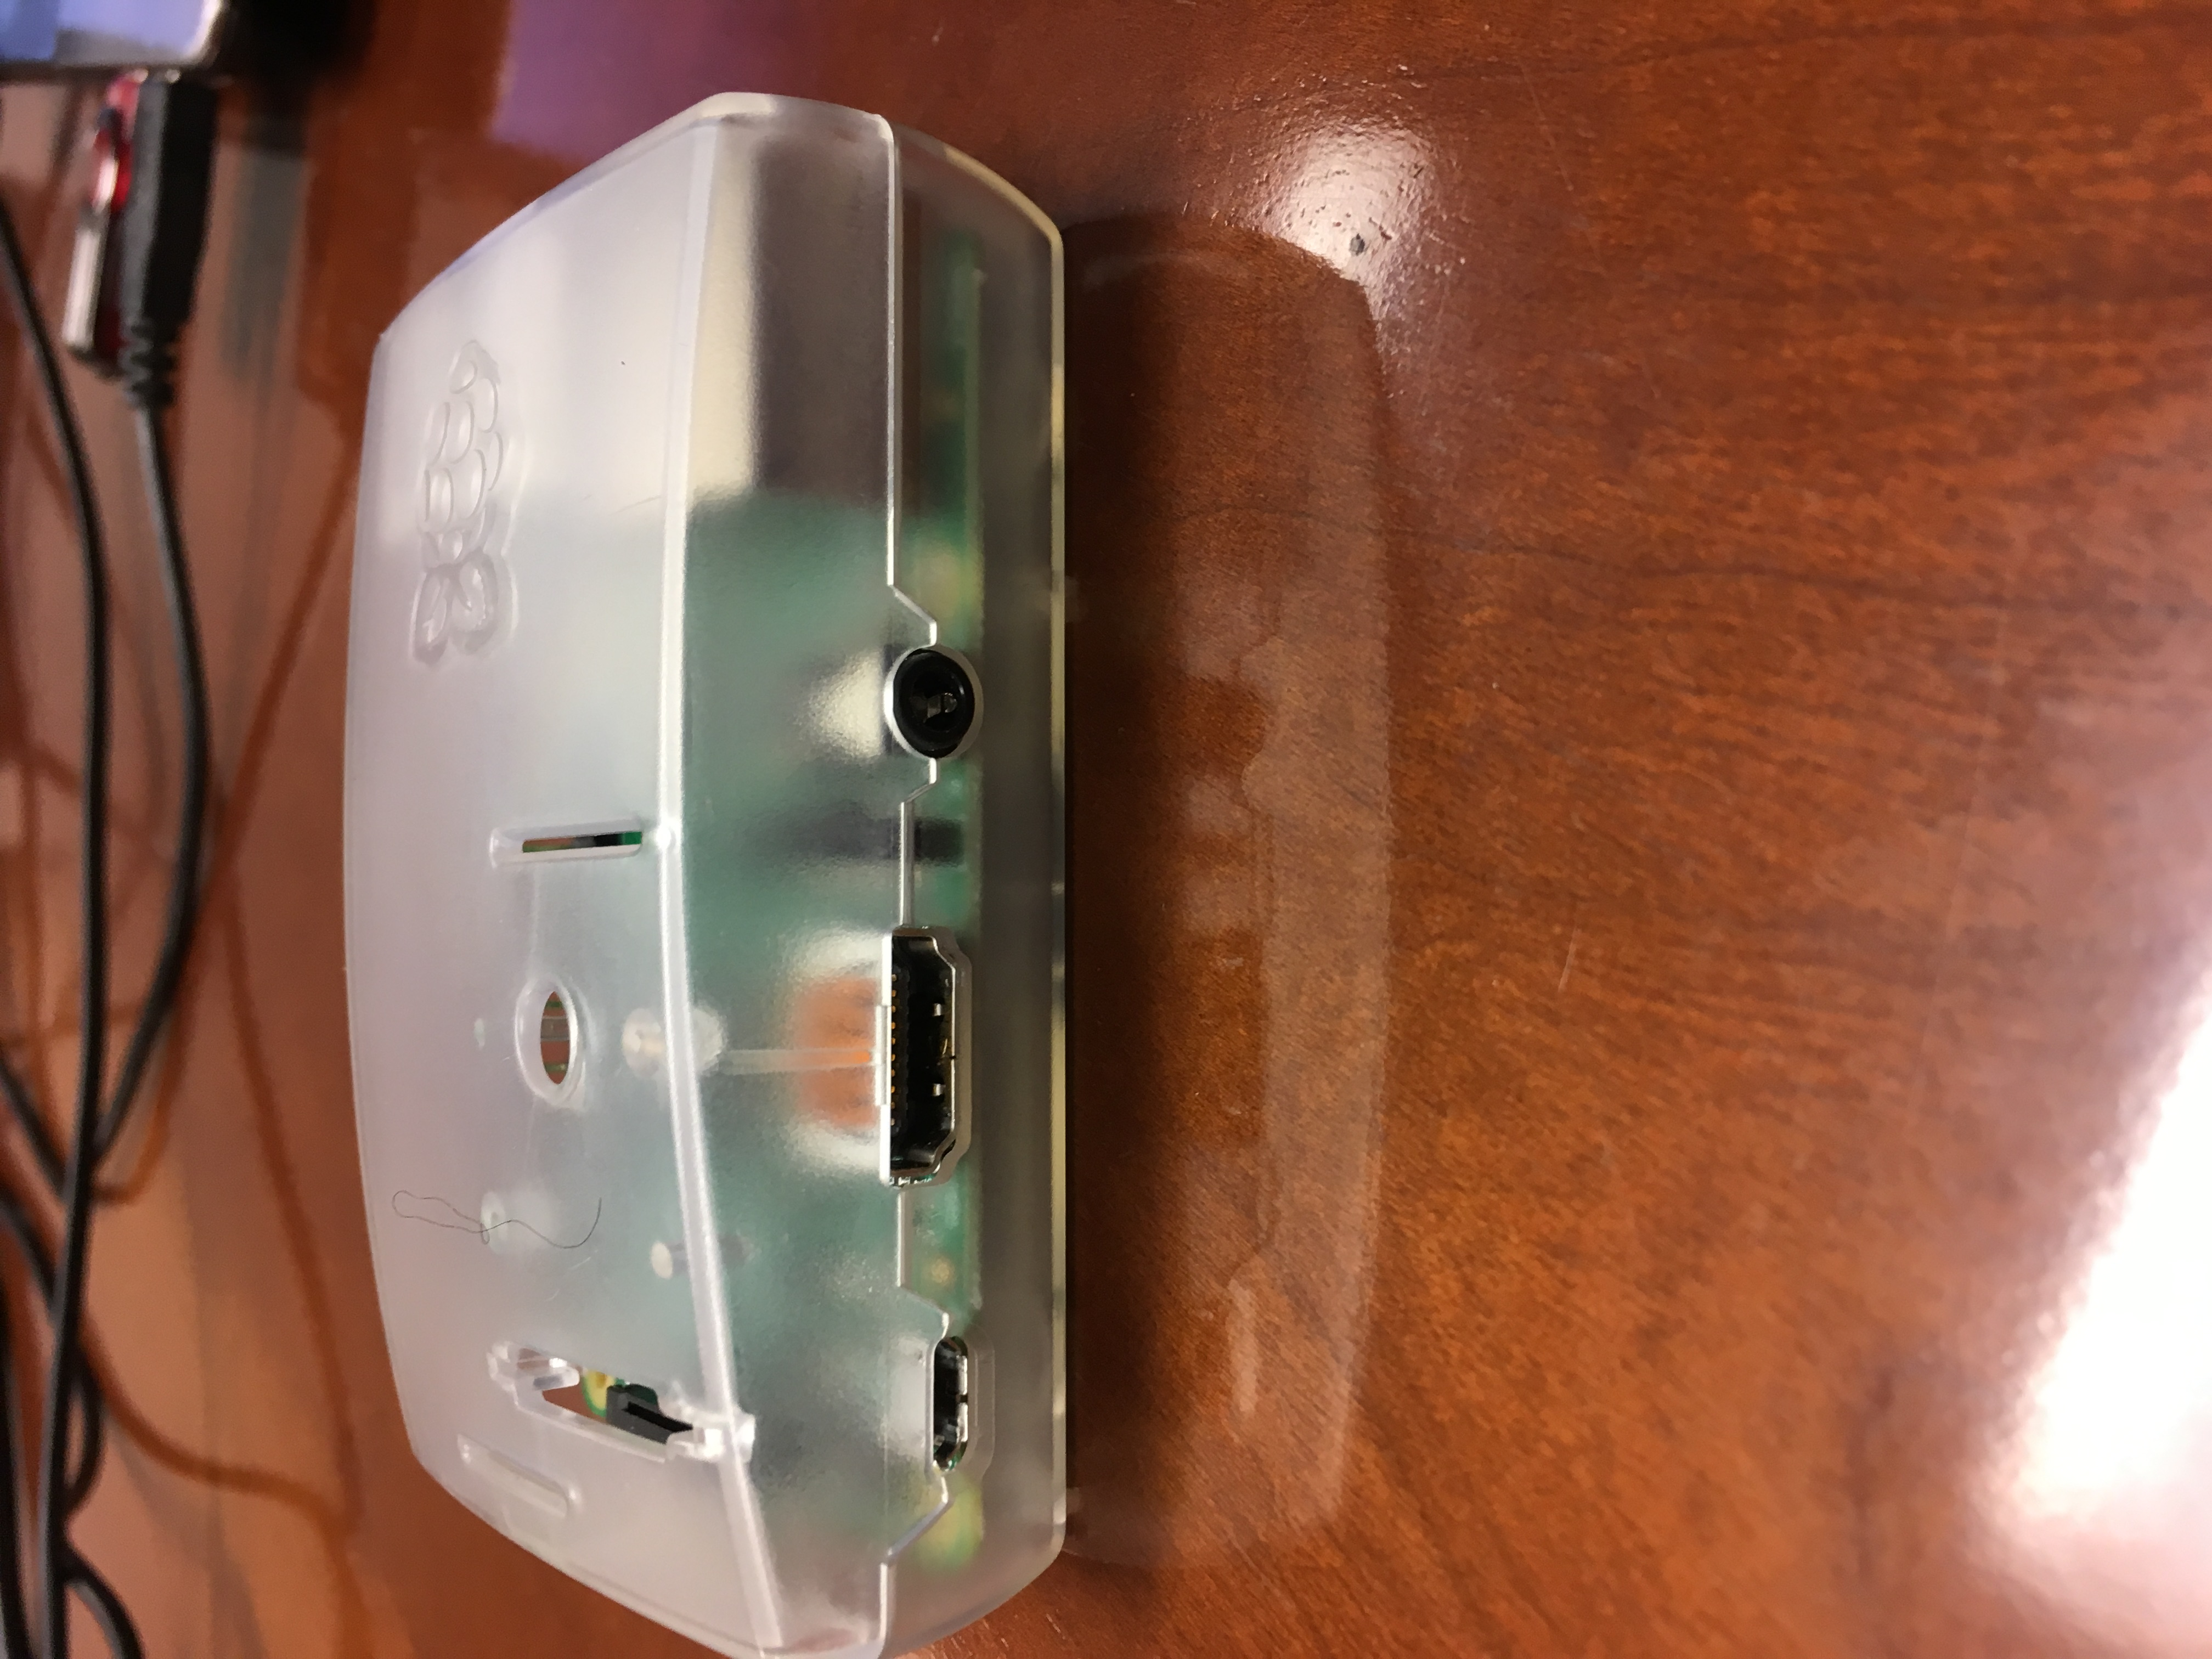
\includegraphics[width=\textwidth]{./figures//IMG_0703.JPG}
    \caption{Raspberry 1}
    \label{fig:r1}
\end{figure}

\end{document}
